\documentclass[10pt,a4paper,titlepage]{report}
\usepackage[utf8]{inputenc}
\usepackage{amsmath}
\usepackage{amsfonts}
\usepackage{amssymb}
\usepackage{graphicx}
\usepackage{color}

\begin{document}
\begin{titlepage}
\author{Rwithik Manoj}
\title{Setting up a Version Control System with Git}
\date{\today}
\maketitle
\end{titlepage}
\begin{center}
\Large{The Local Repository}
\end{center}
\vspace{.5cm}
\par The first step in using a version control system is making the actual repository. Here, I've made a directory named `foss-lab' and converted it into a git repo by using {\color{red} git init} inside the directory. This creates a .git directory inside the repo, which store the details about git. This directory is our local repository. I've also made a README.md file. \newline
\newline
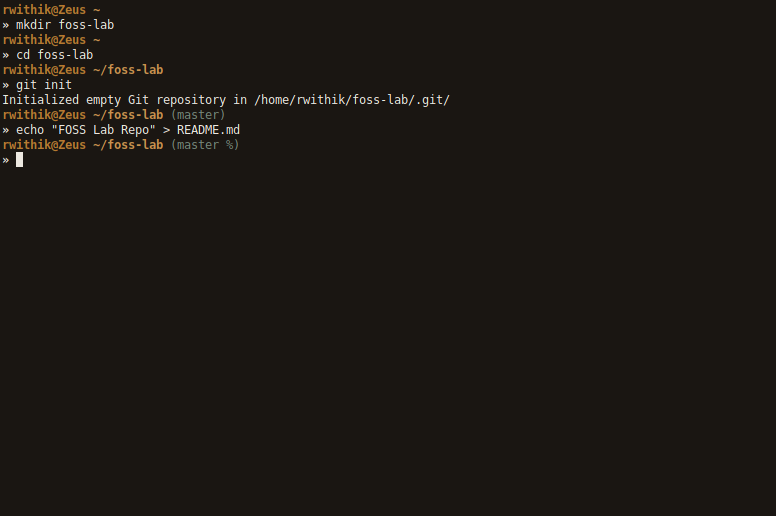
\includegraphics[scale=.45]{../Images/VCS/1.png}
\pagebreak
\begin{center}
\Large{The Remote Repository}
\end{center}
\vspace{.5cm}
\par The local repository exists only on my system. We need to connect it to a remote repository, for any sort of collaboration to be possible. So, I made an online repo at github.com. \newline\newline
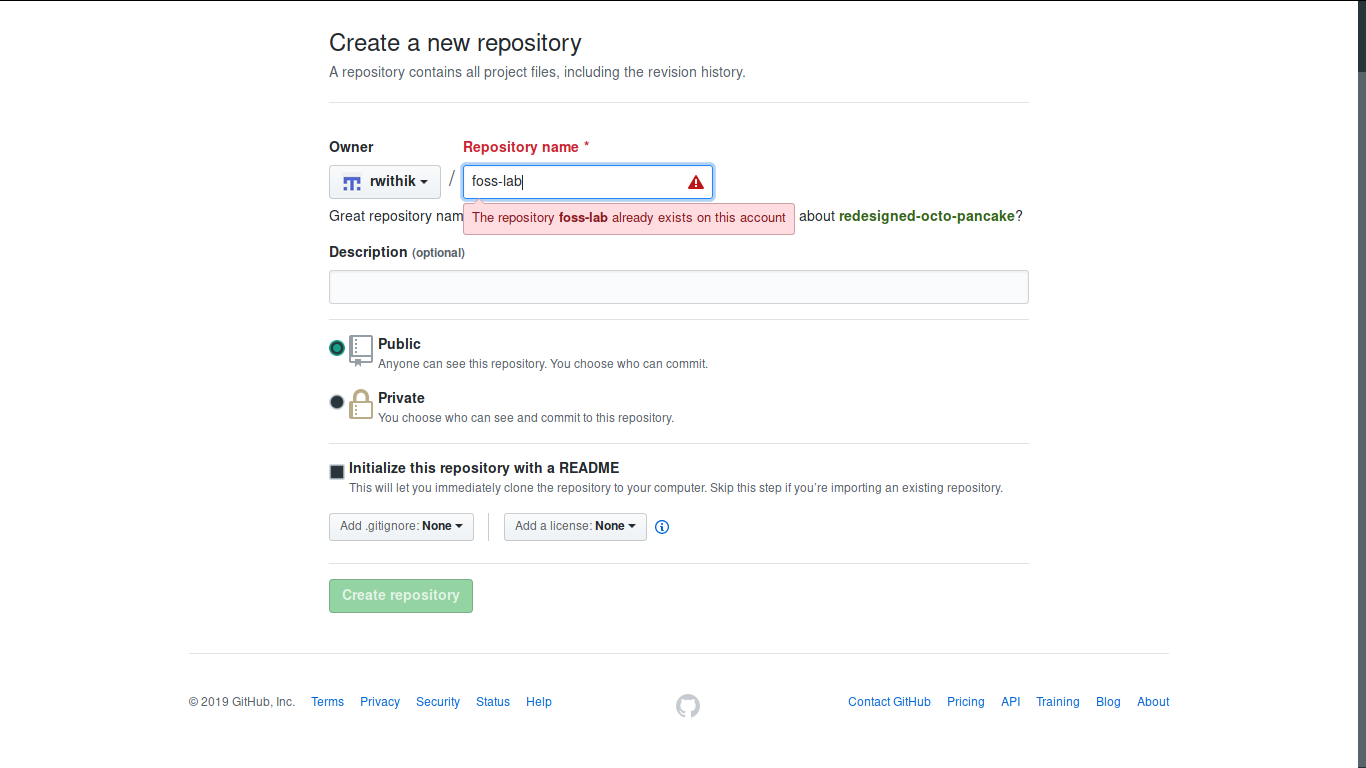
\includegraphics[scale=.25]{../Images/VCS/github.png}\newline
\par Now we need to connect the local repo to the  online repo. This is done using the {\color{red} git remote} command. \newline
Syntax: git remote add origin [URL] \newline\newline
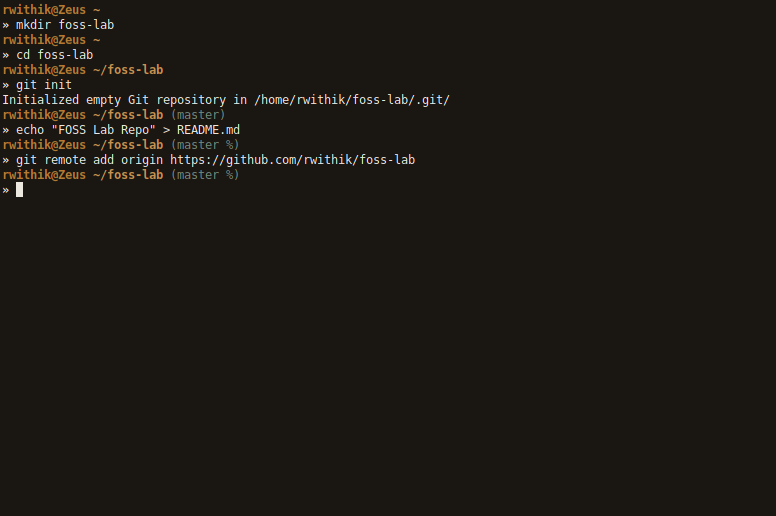
\includegraphics[scale=.45]{../Images/VCS/2.png}
\begin{center}
\Large{Making Changes}
\end{center}
\vspace{.5cm}
\par Any new files or any changes in existing files should be added to the local and remote repositories. This is done with the {\color{red} git add} command. This add the modified and new files to the staging area. Then the files are committed with a commit message using {\color{red} git commit}. This records the changes in the local repo. \newline\newline
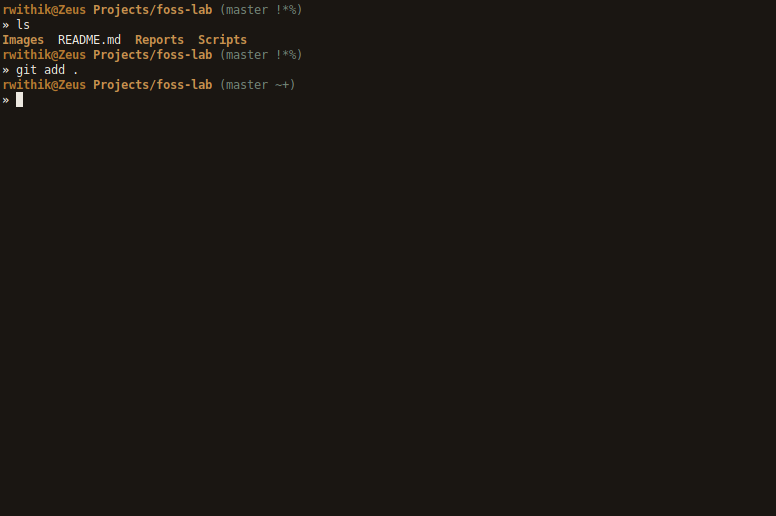
\includegraphics[scale=.45]{../Images/VCS/3.png}\newline\newline
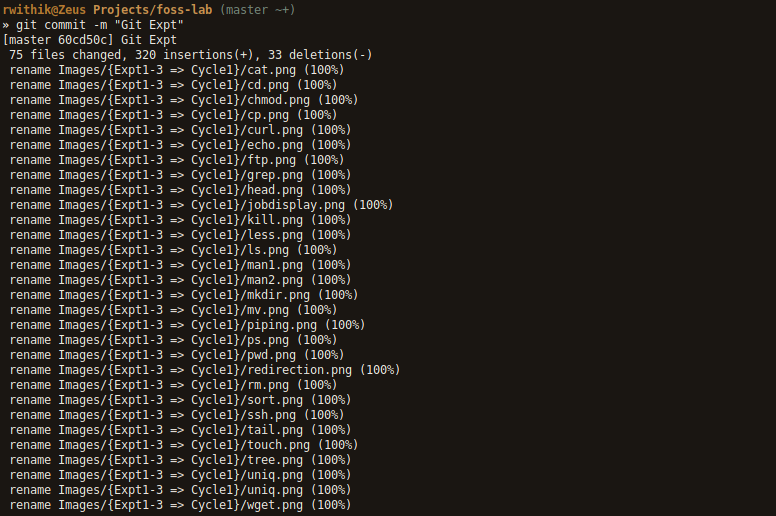
\includegraphics[scale=.45]{../Images/VCS/4.png}
\pagebreak
\begin{center}
\Large{Pushing Changes to the Remote Repository}
\end{center}
\vspace{.5cm}
\par The changes we committed are currently recorded in the local repository. To push these changes to the remote repo, use {\color{red} git push}. In the example given below, origin is the name of the remote, and master is the name of the branch. \newline\newline
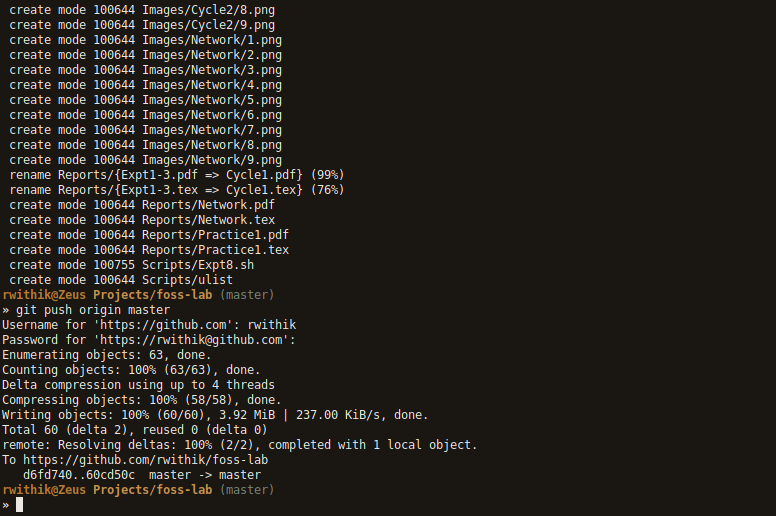
\includegraphics[scale=.45]{../Images/VCS/5.png}
\pagebreak
\begin{center}
\Large{Comparing Previous Versions}
\end{center}
\vspace{.5cm}
\par Use the {\color{red} git log} command to see all the previous changes with their commit messages. \newline\newline
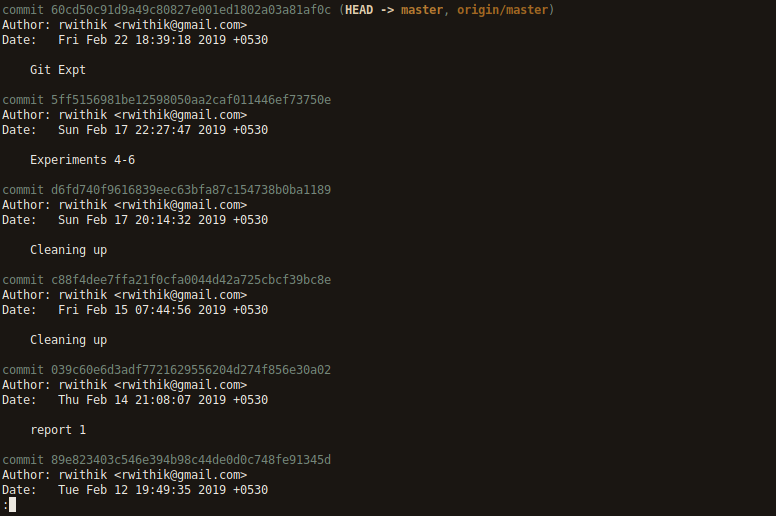
\includegraphics[scale=0.45]{../Images/VCS/6.png}
\end{document}